\documentclass[a4j,12pt]{jsarticle}
\usepackage{semi}
\usepackage{listings}
\renewcommand{\refname}{}
\renewcommand{\lstlistingname}{プログラム}
\begin{document}

%\begin{comment}
%表紙
\begin{titlepage}
\begin{center}
\begin{LARGE}
平成30年度 卒業論文
\end{LARGE}

\vspace{20mm}
\begin{Huge}
シミュレータ教材開発に

関する一提案
\end{Huge}

\vspace{40mm}
\begin{LARGE}
指導教員 須田 宇宙 准教授


\vspace{15mm}
千葉工業大学 情報ネットワーク学科

須田研究室

\vspace{20mm}
1532040 岡本 悠佑
\end{LARGE}
\end{center}


\vspace{35mm}
\begin{LARGE}
\rightline{提出日 2019年2月6日(火)}
 \end{LARGE}
 
\end{titlepage}
\newpage


%目次
\pagenumbering{roman}
\setcounter{page}{1} % ページ番号1
\setcounter{tocdepth}{3}
\tableofcontents
\clearpage
%図目次
\listoffigures
\clearpage
%表目次
\listoftables
\clearpage

%本文
\newpage
\pagenumbering{arabic}
\setcounter{page}{1} 
%緒言
\section{緒言}
近年e-Learningの普及とともに様々なシミュレータ教材の需要が増加している.さらに,パソコンだけでなく,タブレットやスマートフォンといった様々な端末での利用が見込まれ,その利用は学校だけでなく,塾や家庭など幅広い場での活躍が考えられる.

しかし,スマートフォンの性能はPCと比較して決して処理速度が速いとは言えず,従来のシミュレータ教材をそのまま適用するのは容易ではないのが現状である.
しかし,全てのシミュレータ教材を新規で開発した場合その労力は計り知れない.
そのため,ただ処理速度を向上させるだけでなく,変更点が少なく.処理速度を上げることが重要である.

本研究室ではシミュレータ教材にWebWorkerやプログラマブルシェーダーを利用し,GPUを適用させ処理速度の計測を行った.
プログラマブルシェーダによるGPUへの移植やWebWorkerを利用することは処理速度を大幅に向上させるが,記述内容が複雑,増加するため手軽に実装できないことが問題である.

そこでWebWorkerを活用しサブスレッドから直接描画を行うOffscreenCanvasを利用することで処理速度の向上を可能とし,容易に実装を行うことが可能と考える.

本研究ではシミュレータ教材の開発において生産性と処理速度の観点からOffscreenCanvasの有用性を示すことを目的とする.

\newpage
%e-Learning
\section{e-Learning}
e-Learningとはelectronic Learningの略称である.その名の通りコンピュータやネットワークなどの情報技術を扱う学習形態である.e-Learningは1999年11月,アメリカフロリダ州にて開催されたTechLearn1999において初めて使用された.現在CAIやオンラインラーニングなど様々な学習形態が存在する. 

\subsection{e-Learningの定義}
米国の組織学習・人材開発に関する世界最大の会員制組織であるASTD(American SocietY for Training & Development)によると「e-Learningとは,明確な学習目的のために,エレクトロニクス技術によって提供,可能とされた伝達されるあらゆるものである.」と,定義されている.

一般的に情報技術を用いているもの全てをe-Learningと「広義」でとらえる場合と,非同期型オンライン方式を想定した「狭義」である場合とさまざまであり、一概に定義通りではない.テクノロジを活用した学習形態の幅が広がる現在の傾向では「情報技術によるコミュニケーション・ネットワークなどを活用した主体的な学習」を総称してe-Learningと定義するのが一般的である.

\subsection{e-Learningに含まれる学習形態}
e-LearningはIT技術を用いた様々な学習形態を総称して呼ぶ.したがって一言でe-Learningと呼んでも複数の種類が存在する.そこで本章ではe-Learningの種類と特徴・開発の経緯などを紹介する.

\subsubsection{CAI}
CAI(Computer-Assisted Instruction)は1950年代後半,米国で兵員教育の目的として発足.1970年代から80年代にかけて,「講師と受講者が長時間同じ場所に居なければならないという問題を,コンピュータを用いることにより軽減できないだろうか」という,パソコンを教育に活用する学習形態として注目された.CAIはスタンドアローン環境が前提であり,受講者はマニュアル通りの単純な,決められた学習を行う形式だった.そのため受講者のレベルに応じた教育,柔軟なカリキュラムの提示を行えず,効率的な学習を十分に行えなかった.また,ネットワークの利用には至らなかったため,受講者の進捗の確認などは人間が行う必要があった.

1980年代に入るとハードウェアの開発が進み,従来の大型コンピュータで実行されていたCAIがパーソナルコンピュータでも実行可能となり,モデムやスキャナーなどの周辺機器の開発によりメディアとしての能力が向上した.

1990年代にはコンピュータネットワークが発達,個々人の情報リテラシー能力の向上を受け,CBTやWTBが考案,2000年代以降には,これらの概念を活用したe-Learningが盛んに用いられるようになった.

\subsubsection{CBT(Conputer-Based Training)}
CBT(Conputer-Based Training)は,1986年に教育,調査,測定分野の非営利団体であるETS(Esucational Testing Service)が,大学生の能力別クラスの編成用のテストとして利用したことから始まった.当時はットワークが普及していなかったため,CD-ROMの大容量な特性を活かし,動画や音声などを利用したインタラクティブなコンテンツが効果的に利用された.また,受講者管理やコンテンツ配信を行うサーバを必要としないため,比較的容易に導入することが可能だった.しかし.CD-ROMを制作するためのコストと,配布後の修正が難しく,各個人の進捗状況を一括して管理することが困難であった.

その後,1990年代に入り,IT系企業の認定資格試験に利用されたことから大きく発展し,現在では公的要素の強い試験など様々な分野でCBT化が進んでいる.日本国内においても国家試験の一つである情報処理技術者試験で2003年から導入されているように,現在でも学校教育や企業内教育の現場で,幅広く取り入れられている.

\subsubsection{WBT}
1990年代中盤から後半にかけて,ソフトウェアの進化とネットワークの普及に伴い,インターネットやイントラネットなどのネットワークを通して教育コンテンツ学習者に提供するWBT(Web-Based Training)という学習形式である.従来のWBTとCBTとの大きな違いは,ネットワークを介していることである.ネットワークを用いることによる恩恵は以下の3つが挙げられる.

\begin{enumerate}
\item 知識の変化に合わせて教育内容の更新が容易なこと
\item 双方向通信が可能になり,受講者と講師,もしくは受講者同士間のインタラクティブなコミュニケーション,及び受講者の進捗状況の把握が可能になったこと
\item Webは世界標準のプロトコルが存在するため,教材互換性,汎用性,操作性が向上したこと
\end{enumerate}

\subsubsection{EPSS(Electronic Performance Support System)}
EPSS(Electronic Performance Support System)とは,IT技術を活用して,業務中に必要な知識やツールの提供を行うことで,パフォーマンスの向上を支援するシステムのことである.

例としてコールセンターやビデオマニュアルが挙げられる.インタラクティブ学習やパフォーマンス・サポート・システムの分野を専門にしているグロリア・ゲーリー氏によれば「他社による最小限のサポートと介入で,ジュブパフォーマンスが生まれることを可能にするモニタリングシステム,情報,ソフトウェア,支援,データ,画像,ツール,評価の全ての内容に働く人々が簡単にアクセスできる.また,それらを個々人が手元で見ることができ,直ちに必要な内容を入手できる仕組みを持つ,使いやすく統合された電子的環境」と定義している.

CBTやWBTといった,業務から一度離れて学習する形態と比較し,より業務遂行に直結した知識を会得できるシステムであることが特徴であり,近年はより効率化を図るために,これまで活用していた紙のマニュアルを電子化する動きがある.米国においてはユーザのパフォーマンスに合わせた設計を行うことをPCD(Performance Centered Design)と呼び,EPSSと同義として扱われる場合がある.
\subsubsection{Knowledge Management System}
Knowledge Managementとは,個人の持っている知識,情報を組織で共有し,コミュニティ全体の創造性を向上させるための手法である.個人の持つデータだけでなく,経験やノウハウを含んだ幅広い物を指す.

Knowledge Managementとe-Learningは独立したものと扱われることが多かった.しかし,米国でe-Learningの分野においても,マニュアルの理解や受講者間での知識の共有や生成の場を設けることの重要性を訴えられる様になった.そのことが実現した場合e-LearningとKnowledge Managementの区別がなくなるため,両者を融合し,e-Learningの一環として捉えるようになった.

\subsubsection{Blended Learning}
Blendes Learningは,e-Learningと集合研修を組み合わせた形態ことである.

それらの組み合わせは,他者からの刺激を受けることで学習意欲の向上,相互作用をによって理解促進,知識の整理が行えるという利点がある.
\begin{description} 

\item[e-Learnig + 集合研修]\mbox{}\\ 
事前学習を済ませた後に,教室でインタラクティブな学習を行う

\item[e-Learnig + 集合研修]\mbox{}\\ 
事前学習と教室研修を行い,その後にバーチャルクラスで学習を行う

\item[集合研修 + e-Learnig]\mbox{}\\ 
集合研修後にフォローアップのためにセルフ学習を行う

ディスカッションバーチャルクラス,チュータからのメンタリングを含む
\end{description}
このように様々な形態が存在するが,e-Learningに適した内容化を見極める必要である.
\newpage

%効果
\subsection{e-Learningの効果}
e-Learningには様々な形態が存在するが,学習形態ごとに違いがあるが,e-Learnigという大きな枠組みで考えたときのメリットとデメリットをまとめる.
\subsubsection{e-Learningのメリット}
\begin{large}受講者のメリット\end{large}
\begin{enumerate}
\item 場所と時間に制限がない
\item 受講者のレベルや習熟度に合わせたコンテンツの提供できる
\item 研修終了後に受講者間や講師との間でインタラクティブなコミュニケーションが可能
\item 世界標準のプロトコルを用いることで,教材の互換性,汎用性,及び操作性が向上
\item 予め筋道を立ててシステムを組むため,全体の筋道が決まっており,一括して見やすい
\item 場所の移動を省くことが可能なため,時間とコストを削減できる
\item 最新の情報を安価で早く入手し,学習することができる
\end{enumerate}

\begin{large}制作側のメリット\end{large}
\begin{enumerate}
\item 集団教育と比較すると安価に提供できる
\item マルチメディアを用いたインタラクティブな教材の制作が可能
\item 学習の進捗状況をリアルタイムで把握することができるため,管理が用意
\item 知識の変化に合わせ,最新の内容に更新した教材の把握が容易
\end{enumerate}

\subsubsection{e-Learningのデメリット}
\begin{description} 

\item[(1)コンピュータ,またはインターネット環境が整っているところでしか学習できない]\mbox{}\\ 
本などの資料は,持ち運びが容易なため,電車の中などで資料を持ち込むことや書き込むことで学習することが可能だが,e-Learningでは難しい.しかし,小型の端末などで学習を行えるソフトがリリースされており,以前と比べるとその欠点は薄れつつあるといえる.

\item[(2)就業時間中の学習を公認する必要がある]\mbox{}\\ 
集合研修は,会社がその時間の学習を公認しているが,書籍での学習は就業時間外として扱われることが多く,自主学習形態をとることが多い.しかし,e-Learningはインターネットが使えるコンピュータで学習することが一般的であり,セキュリティ上社外からのアクセスは禁じられていることが多く,学習するには社内で行う必要がある.その場合就業中か,仕事を終えて自分の席で学習することになる.自分の席で学習する場合,他者の目にはばかられ,思うような学習は難しいと思われる.就業時間中の学習は多くの企業で公認されにくいため,教材をリリースしても誰も学習しないという状況も多い.

\item[(3)システム投資コストがかかる]\mbox{}\\ 
e-Learningを使用する環境を構築するには教材を制作するだけでなく,サーバ管理コストやコンテンツ維持コストや補助的サーバなどが挙げられる.また,レポート提出や質疑応答システムと統合した環境を整えるとそれなりに費用がかかってします.システムの投資コストが従来の教育コストより高くなってしまう場合,e-Learningのメリットが無くなってしまう.

\item[(4)コニュニケーションや,体で覚える技術教育には向かない]\mbox{}\\
実際に対話を行う集合研修に対し,e-Learningは成約が多い.しかし,誰かが一方的に話すタイプの集合研修と比較すれば,この弱点は解消されたといえる.

\item[(5)シミュレータ搭載が困難]\mbox{}\\
 現在実用化されているe-Learning教材のなかで,文系科目に該当する大学などで多く実用化されている.その背景に容易に制作が可能なことが挙げられる.容易に作成できることからコンバータを用いることが多いが,コンバータはシミュレータやアニメーションに対応されておらず,実験などの補修学習が要の理系科目において十分な効果を期待することはできない.
\end{description}
\newpage
%シミュレータ教材
\section{シミュレータ教材}
\subsection{シミュレータ教材の定義}
シミュレータ教材とはシミュレーションを行う教材のことである.

現実世界の問題はシステムが複雑で予測が困難な場合が多く,実システムで試すにはコストや時間がかかるといった場面が多く存在する.
しかし,コンピュータ上に現実世界を再現することにより,実際のシステムの制作,変更することなく様々な条件下の環境を再現,システムの挙動を調べることができる.このコンピュータ上に現実世界を仮想的に制作するシステムをシミュレータと呼ぶ.

したがって,シミュレータ教材とは様々な条件下の現象を実際に生成することなく再現することで,対象を視認,理解させるための教材である.

一般的には,航空シミュレータや音響シミュレータなど,シミュレーションの結果を体験させるためのシステムを指すことが多いが,本研究では,コンピュータ上で動作し,ブラウザ上でパラメータを変更させ,その結果を同じブラウザ上で確認できるソフトウェアのことを指す.

%FTDT法
\subsection{FDTD法}
音場のシミュレーションは大きく分けると定常解析手法と非定常解析手法の2つに分類される.定常解析手法とは対象が定常状態に達したときの音場や位相を計算する手法である.音波は時間とともに変動するが定常状態のため時間に依存することなく空間分布が求められる.

一方,非定常解析手法は時間によって変化する場を取り扱う.したがって音圧などの物理量が時間と共に変化する場を扱うため,波形そのものの計算が得意である.

本章では本研究に使用し,音響のシミュレータにおいて度々用いられる非定常手法の一つであるFDTD方について論じていく.

\subsubsection{FDTD法の概要}
FTDT(Finite Difference Time Domain)法は,1966年にK.S.Yeeによって提案された.K.S.Yeeはマクスウェル方程式が電解と磁界の連立方程式であることに着目し,中心差分に電磁界の時間及び空間配置を考案した.後に多くの科学者によって発展し,現在では電磁波の支配式を求めるだけでなく,流体力学や熱工学だけでなく波動光学にも用いられることが多くなった.
\newpage

\subsubsection{計算方法}
物体に力を加えると物体は移動する,それと同様に空気も力が加わると動きが生じる.それはニュートンの第2方式,すなわち,運動方程式で記述される.空気には物体に動きが加わることによって生じる圧力と,運動に依存しない圧力が存在し,音響において前者を音圧,後者を大気圧と呼ぶ.音波の伝搬する空間を音場と呼ぶ.

ある空間においてX,Yの直交座標の寸法がそれぞれ$\Delta X$,$\Delta Y$とし,密度をρ,音圧を$p$とし,それぞれの変異を$u_X$,$u_Y$とする.$\Delta X$が微小であると仮定したときのX方向の運動方程式は
\begin {eqnarray}
\label{eq:X}
\rho \frac {\partial t^2} {  \partial ^2 u_x } = - \frac { \partial p } { \partial x} \
\end{eqnarray}
Y方向も同様に
\begin {eqnarray}
\label{eq:Y}
\rho \frac {\partial t^2} {  \partial ^2 u_y } = - \frac { \partial p } { \partial y } \
\end{eqnarray}
と表される.体積弾性率を$k[\mathrm{N/m^2]}$としたときの音圧に関する連続方程式は
\begin {eqnarray}
\label{eq:w}
p = -k ( \frac { \partial u _ x } { \partial x } + \frac { \partial u_y } { \partial y } \ )
\end{eqnarray}
となる.
式(\ref{eq:X}),(\ref{eq:Y}),(\ref{eq:w})を物理現象を方程式化した式,すなわち,支配式として音場の解析を行う.これらの式を時間微分した式を以下に示す.

\begin {eqnarray}
\label{eq :  X-2}
\rho \frac{ \partial v_x } { \partial t } = - \frac { \partial p }{ \partial x }
\end{eqnarray}
\begin {eqnarray}
\label{eq :Y-2}
\rho \frac{ \partial v_y } { \partial t } = - \frac { \partial p }{ \partial y }
\end{eqnarray}
\begin {eqnarray}
\label{eq :  w-2}
\frac{ \partial p } { \partial t } = - k ( \frac { \partial v_x }{ \partial x } + \frac { \partial v_y }{ \partial y } ) 
\end{eqnarray}
となる.

音圧は時間と共に連続的に変化するが,コンピュータは連続の関数を扱うことができない.したがって,空間や時間を細かく区切ることで,連続な関数に見せる必要がある,このことを離散化と呼ぶ.
また,空間に関する区切り幅を空間離散化幅,時間に関する区切り幅は時間離散化幅と呼ぶ.区切りごとの離散的な値を参照点と呼ぶ.

FTDT法における音圧の離散化は,隣り合う参照点がそれぞれ$\Delta$X,$\Delta$Yの空間離散幅を持ち,$\Delta$tの時間離散幅を持つ.参照点からX,Y方向に関して何番目の音圧参照点かをI,Jを空間ステップと呼ぶ.何番目の時間参照点であるか$n$を用いて表すと,$(n-0.5)\Delta t\mathrm{[s]}$であり,この$n$を時間ステップと呼ぶ.

Xに関する偏微分係数を
\begin {eqnarray}
\label{eq :X-3}
- \frac { \partial p }{ \partial x }|_{ x=x_0} = \lim_{\Delta x \to 0} \frac{p|_{x=x_0+ \frac {\Delta x}{2} -p}| _{x=x_0} - \frac{ \Delta x}{2} }{ \Delta x} \verb|~| \frac{p|_{x=x_0+ \frac {\Delta x}{2} -p}| _{x=x_0} - \frac{ \Delta x}{2} }{ \Delta x}
\end{eqnarray}
のように近似する.
式 \ref{eq :X-3}を式 \ref{eq : X-2}に適用し,空間ステップを$i+0.5$,jの位置,空間ステップNの時刻としたとき

\begin {eqnarray}
\label{eq:X-4}
\rho \frac{ v_x^{n+0.5}( i+0.5, j ) -v_x^{ n-0.5 }( i+0.5,j ) }{ \Delta t } = - \frac{ p^n( i+1 ,j ) -p^n( i,j ) }{ \Delta x }
\end{eqnarray}

と近似できる.空間微分にも時間微分にも式\ref{eq :X-3}と同様の近似を用いることが可能となり,これがFTDT法の特徴の一つである.式\ref{eq :Y-2}も同様に近似値を求めることができる.

\begin {eqnarray}
\label{eq:Y-4}
\rho \frac{ v_y^{n+0.5}( i+0.5, j ) -v_y^{ n-0.5 }( i+0.5,j ) }{ \Delta t } = - \frac{ p^n( i+1 ,j ) -p^n( i,j ) }{ \Delta y }
\end{eqnarray}


時間ステップN-0.5を過去,Nを現在,N+0.5を未来の状態と考えれば,過去のX方向の速度$v_X$の値と現在の値から未来の$v_X$の値を求めることができる.
最も時間ステップが大きい項のみ左辺に変形し,初期の粒子速度分布と音圧分布の1組がわかれば,全空間ステップにおいて変形した式を交互に計算することで求めることが可能である.初期時刻の場の業態を表す条件のことを初期条件と呼ぶ.時間が進むごとに次々と変化することを時間発展と呼び,初期状態から時間的な順序を追って場の上程を求めることを逐次計算と呼ぶ.

\newpage
\subsection{シミュレータ教材のメリット}
シミュレータを使用することに得られるメリットを以下に示す.
\begin{enumerate}
\item コンピュータで疑似体験

シミュレータ教材とは,現実の物理現象をモデル化し,コンピュータ上で計算することで,模擬体験できる藻である.仮想環境の中での学習により,従来では考えられない程の学習効果を得ることができ,学習者の意欲向上に繋がると考えられる.
\item 等しく均一の条件で学習が可能

学習者自身が,実験の条件や変数を変えながら実験に参加することが可能である.実験変数の変更を安全に,何度でも変更することが可能なため,繰り返し学習が可能となり,学習者は全員均一の条件で学習できる.
\item 安全性

シミュレータ教材により学習者は,教室内で費用,時間のかかるものや.危険で簡単に実施できない実験を疑似体験することができる.
\end{enumerate}

\subsection{シミュレータ教材のデメリット}
シミュレータ教材は通常,全ての現象を思考要素とせず,対象要素を絞り込むことにより,要素が現象に与える影響を検証することが目的である.したがって,結果が不確定な事象を検証することは極めて困難である.

コンピュータを用いた積算によるシミュレートは,基本線形近似による計算のため,非線形を含む自然現象をシミュレートする場合は必ず誤差が生じる.良好な結果が得たければ,誤差見積もりが重要になる.

そして,シミュレータ教材を使うにはシミュレータ教材を作る必要がある.開発者はシミュレータを開発するためのソフトウェアを保持した状態で,プログラミングの知識や主題についての専門的な知識が要求されるため,開発者が限定される.
\newpage
%プロセッサ
\section{プロセッサ}
本章ではプロセッサ,CPUやGPUの歴史や相違点といった内容を解説する.
%CPU
\subsection{CPU}
CPUとはCentral Processing Unitの略称である.人間でいう頭脳と例えられることが多いパーツである.本章ではその概要と歴史について記す.
\subsubsection{CPUの概要}
CPUの外見は大きさが数[cm],厚さ数[mm]で,容器に覆われている.裏面には外部との接続のため,数多くのピンが設けれらている.このピンを介して,CPUはプログラムを読み込み実行するのである.

CPUの役割はメモリやハードディスク,マウスなどからデータを受け取り,計算,判断をし,その結果をディスプレイやメモリ,ハードディスクに送り出すことである.
それらの命令を実行するためには図\ref{fig:cpu}のように複数の演算ユニットが必要になる.
CPUは,外部から供給されるクロック信号に合わせて内部動作を進め,その信号は数[GHz]と非常に高い.

\begin{figure}[htbp]
 \begin{center}
  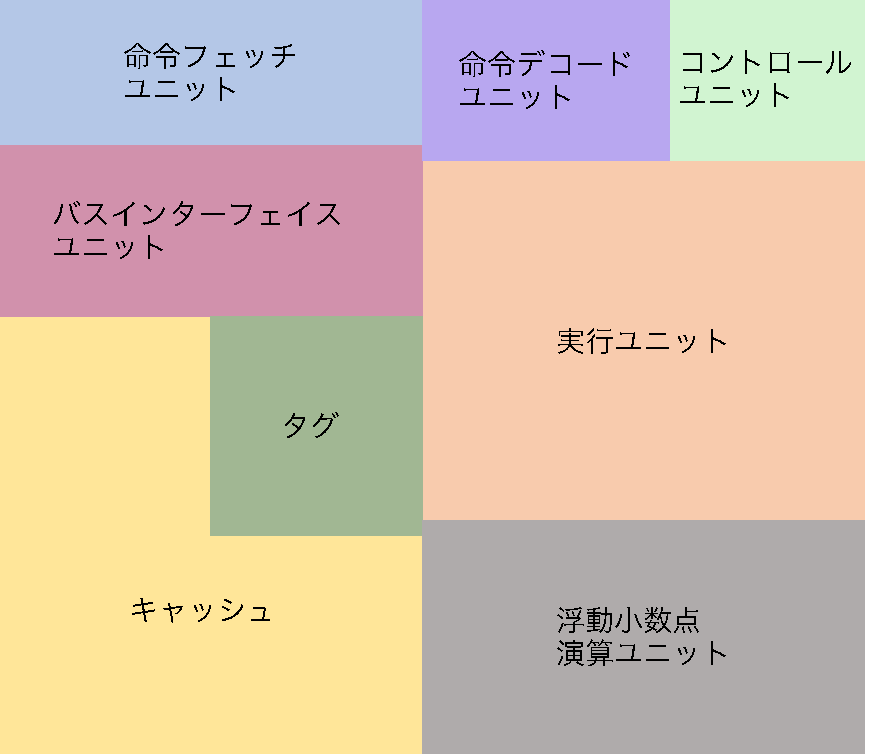
\includegraphics[width=70mm]{CPU.pdf}
 \end{center}
 \caption{CPUの内部構造の略図}
 \label{fig:cpu}
\end{figure}

\subsubsection{CPUの歴史}
パソコンが誕生する前のコンピュータは非常に高価なため,個人が所有できる代物ではなかった.しかし,1971年にインテルが4ビットCPU4004の開発に成功したことにより,以前より手軽にコンピュータを入手できるようになった.1974年には更に性能が向上した8ビットCPUを開発した.同年MITS(マイクロ・インスツルメンテーション・テレメトリ)が本CPUを利用したコンピュータALTAIR8800を販売した.8080は汎用性が高く,様々な製品に組み込まれた.

1978年に16ビットCPUの8086が登場した.その後,80286,80386,80486そして,Pentiumへと進化していった.これらの特徴として上位互換性があることである.つまり,以前に作られたOSやアプリケーションを動かすことができる.この一連のCPUはCISC(CompleX Instruction Set Computer)タイプのCPUと分類される.実行可能な命令はCPUごとに異なり,CPUが実行可能な命令を全部合わせて命令セットと呼ぶ.CISCは複雑命令セットコンピュータと呼ばれ,それぞれの命令の機能が複雑かつ強力に作られている.

1980年RISC(Reduced Instruction Set Computer)が発表された.RISCは命令を使用頻度の高いものに限りられ,基本設計がシンプルなのが特徴である.

RISCは数多くのメーカのCPUに採用されており,1985年にSun MicrosystemsがSPARCを開発し,1986年にはARM社から低消費電力を重視したARM2とPA-RISKの最初の実装であるT1を搭載したHP 3000が登場した.その後1990年にIBMが16ビットのRISCマイクロプロセッサのPOWERを発売した.

一方,CISCタイプのCPUのpentiumを開発していたIntelも RISCベースのCPUであるi960を発売していた.

その後,パソコンにおいて従来CPUとのの互換性を保持しつつ,RISC技術を取り入れたインテルが優位に立ち,ワークステーションにおいてはRISC CPUに軍配が上がった.

1990年代に入ると業務用向けに64ビットのCPU MIPS R4000が登場した.家庭用では1994年にソニーから発売されたPlayStationにR3000が搭載されるなど32ビットへの移行が進んでいた.

64ビット向けワークステーションの市場はRISCが占め,32ビットの市場もAMDやCyrixなどが競い合っていた.そこでIntelは家庭用向けの64ビットCPUの命令セットを発表しが,開発が遅延したことや,POWERなどの競合プロセッサの性能向上により普及することはなかった.

1993年にインテルがPentiumシリーズを発売した.初期のクロック周波数は60MHzだった.その後200MHzまで向上する.

1990年代後期にはサーバ向けCPUの64ビット化が一区切りし,高クロック数,マルチプロセッシングへと変化していった.

2000年に入りAMDがAthlonを発表し,最大周波数1GHzになった.同年インテルはAthlonに対抗してPentium4を発表し,動作周波数は1.3GHzまで向上した.

2002年にサーバ分野でマルチコアCPUが導入された.翌年パソコン分野において64ビットのCPUが登場した.

2004年に周波数向上の限界に突き当たった.周波数を向上させることにより,消費電力が増加した.
そこでインテルは2005年に1つのパッケージに2つのCPUコアを実装したCPUを開発,Pentium Dの登場である.このCPUがマルチコア化への先駆けとなった.同年AMDからマルチコアのAthlon 64 X2が発表された.AMDはクロック数が1GHzへ到達した時点で処理効率を重視したCPUを展開した事により,デュアルコアへの拡張を意識した設計を可能とした.この頃から消費電力あたりの性能が重視されるようになった.
サーバ向けのCPUではワンチップで数十スレッドを実行するCPUが現れた.相対的に低いクロック数で性能を引き出しやすいSIMD(single instruction multiple data)の性能に重点が置かれた.

\subsubsection{CPUの処理方法}
\begin{Large}
パイプライン
\end {Large}

CPUで処理を行う時プログラムはフェッチ,読み込み,実行,メモリに書き込みを繰り返している.処理を行う時,これらを順番に実行するが,同時に一つの処理しか行えない.そこでステージ数を増やすことで複数の命令を実行可能とした.Pentium4ではステージを増やすことで高クロック化させた.

\begin{Large}
SIMD
\end{Large}

SIMDとは(Single Instruction Multiple Data)の略称である.SIMDは1回の命令で複数のデータに対する処理を同時に行う演算装置設計手法である.同一の処理を大量に行わなければならないマルチメディアの処理などに向いている.

Pentium向けに開発されたMMXや,Pentium\UTF{2162}から実装されたSSE(Streaming SIMD Extensions)などがある.

%GPU
\subsection{GPU}
GPUはGraphics Processing Unitの略称である.GPUは画像処理,大量の計算を行うことを目的として開発されたハードウェアである.しかし,近年はその処理能力の高さからディープラーニング等画像処理以外の分野での活躍も多く見られるようになった.
本章では.GPUの概要から歴史,処理の仕方について述べる.


\subsubsection{GPUの概要}
GPUは画像処理を行うことを目的としている並列演算ハードウェアである.本来GPUは画面の出力やそれに付随する演算を行う.家庭用のパソコンにでは画面の出力の他にリアルタイムで大量の計算を必要とする3Dゲームなどを行うのに役立っている.

しかし,その高い処理能力を画像以外に活かすためにNVIDIAはグラフィックス処理以外の演算を行わせるようにしたGPGPU(General-Purpose computing on GPUs)の開発環境CUDAを一般公開した.GPGPUの研究が注目を浴び,現在ではその高い処理能力を活かしディープラーニングに広く普及している.

一般的にGPUとは,図\ref{fig:gpu}のようなビデオカード(グラフィックボード)と呼ばれるハードウェアとして販売されている機器を指し,ビデオカードとLSIチップを区別しないで呼ばれることが多い.

\begin{figure}[htbp]
 \begin{center}
  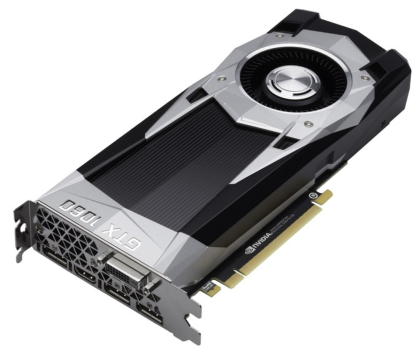
\includegraphics[width=50mm]{GPU.pdf}
 \end{center}
 \caption{グラフィックボード}
 \label{fig:gpu}
\end{figure}

\subsubsection{GPUの歴史}
1970年代に入り大型のコンピュータのサイズダウンが行われ,ミニコンという種類が登場,低価格帯のCPUによる一般向けのコンピュータ,パーソナルコンピュータ(パソコン)が登場した.世界最初のパソコンと呼ばれているアルテアにはモニタがなく,コンピュータの状態をLEDで表示するにとどまった.モニタに対応したのアップルのApple\UTF{2160},Apple\UTF{2161}だった.
当時のパソコンには,メモリ上にビデオ表示用の領域があり,後にVideo RAM(VRAM)と呼ばれるようになった.VRAMの領域を書き変えることで画面に出力ができた.

1990年代に入るとパソコンでもGUIの環境が整ってきた.GUIが発展すると以前の640×400ドットより広い描画範囲を必要とした.そのため,ユーザの間ではビデオカードを用いて描画領域を拡張させる動きがあった.Windows95が発売のころには,ビデオカードが含まれるパソコンが標準となった.

1995年に3dfXから3Dの処理に特化したVoodooが発売された.当時は家庭用のパソコンとアーケードゲームのグラフィックに差が存在したが,Voodooの登場により家庭用のパソコンもアーケードゲームに匹敵する品質を実現させた.

1997年にはCYriXからオーディオチップとグラフィックチップが1つのチップセットに統合されたMesiaGXが発売されるなど,複数のチップを統合した製品が登場する.グラフィックス機能が貧弱であったり,低価格帯をターゲットとしてたため利用できるCPUの性能にも限度があり,普及しなかった.
しかし,1999年にIntelから発表されたIntel 810チップセットは,2D描画性能は十分な性能を有したため,オフィス処理やブラウジングなどには十分な性能であった.また,同設計で多様なCPUを採用した製品を開発しやすかった.グラフィックカードが不要なことから小型なパソコンの設計が可能となり,グラフィックチップが組み込まれたチップセットが普及した.

1999年にNVIDIAから高い3Dの演算能力を有するGeForce256が発売された.GeForce256の特徴は3D演算用のハードウエアが搭載されたことである.それまで3D専用ワークステーションでしか行えなかった分野がパソコンでも行えるようになった.CPUが通常の演算を行うことから,グラフィックの演算処理を行うハードウエアをGPUと呼ぶとNVIDIAが提案,その呼び名が定着した.

2001年にはGPUの固定機能パイプラインであるシェーダ処理がプログラム可能になった.しかし,アセンブラが基本として扱われたため敷居は非常に高かった.その後,シェーダのプログラムを書くための高級言語が登場,3Dグラフィック以外の演算も行われるようになった.演算ユニットを汎用化させる統語柄シェーダーアーキテクチャが登場,GPUにおける汎用演算GPGPUの発展,普及へとつながっていった.

2010年に入るとCPU分野ではマルチコアを搭載するだけでなく,画像出力専用回路としてGPUコアを統合した製品の提供を行った.それまで行われていた画像データを外部メモリ空間へ転送するといった処理は不要になった.

\subsubsection{GPUの処理方法}
GPUを構成するプロセッサの最小単位はスカラプロセッサである.スカラプロセッサはCPUと比較して,算術計算やロジック処理等,限られた機能しか持ち合わせていない.スカラプロセッサはCPUのプロセッサと違い命令デコードが存在しない.

ストリーミングマルチプロセッサは複数のスカラプロセッサを内蔵させたプロセッサである.従来は8個であったが,現在では数が一定ではなくなった.ストリーミングマルチプロセッサには複数のスカラプロセッサを制御するユニットが搭載されている.また,命令デコード機能が含まれている.そのときマルチプロセッサに伝達される内容は同じ内容となっている.

スカラプロセッサ上で動作するプログラムの単位として,スレッドがある.スレッドは32スレッドごとに動作する.
GPUは1つの命令で複数のスカラプロセッサが動作するが,開始のタイミングは同時でなく、プログラムごとに1クロックのズレが生じる非同期の動作である.したがって,プログラム上で同期を行うことが重要となる.

\subsubsection{プログラマブルシェーダー}
プログラマブルシェーダーはMicrosoftが開発したゲーム及びマルチメディア処理用のAPIであるMicrosoft DirectX 8から導入された技術である.CGにおいて光の当たり具合などを調整して各画素の色を変化,陰影をつける処理であるシェーディングをGPU上のプログラムとしてリアルタイムに実行する技術である.

DirectX 7までは内部で行われた描画処理の順番や処理は固定であったが,DirectX8移行はプログラムで自由に設定を変更できるようにした.

プログラムでシェーディングが可能になったことにより,ハードメーカーが開発されるグラフィック表現に対応したハードウェアを逐一実装する必要がなくなった.また,プログラムを利用することで画面効果を試験的にGPU上で再現することが容易になったことにより表現力が向上した.

プログラマブルシェーダー向けの言語のことをシェーディング言語と呼ぶ.

主なシェーディング言語を以下に示す.
\begin{description}
\item {GLSL}\mbox{}\\ 
GLSLはOpenGL  Shading Languageの略称である.GLSLはC言語をベースとして開発された言語である.2003年にOpenGL1.5の拡張機能として導入され,翌2004年にOpenGL ARBによって策定され,OpenGL2.0に導入されることとなった.
た.

\item	{DirectX}\mbox{}\\ 
DirectXはMicrosoftが開発したゲーム・マルチメディア処理用のAPIである.
1995年にWindows 95用にWindows Game SDKとして登場したのが始まりである.定期的にバージョンアップされており現在は2015年にリリースされたDirectX 12が最新である.

\item	{CUDA }\mbox{}\\ 
 2006年にNVIDIAから発表された並列コンピューティングアーキテクチャである.CUDA(Compute Unified Device Architecture)はそれまで画像処理や出力が主な目的だったGPUに汎用処理をさせることを目的に開発された.専用のコンパイラやAPIなどが提供されている.
\end{description}
\newpage

%HTML
\section{HTML}
HTMLとはHYper TeXt Markup Languegeの略称であり,ウェブ上のドキュメントを記述するためのマークアップ言語である.HTMLで制作されたドキュメントは異なるドキュメントへのハイパーリンクを設定でき,リストや表などの作成を行うことができる.また,CSSやJavaScriptなどを別ファイルから読み出すことが可能である.
\subsection{特徴}
HTMLの特徴はハイパーテキストを利用した相互間文章参照のフレームワークである.文章中にURLを用いて他の文章へリンクを記載することで,指定された他の文章を表示させることが可能である.

HTMLはマークアップ言語であるが,マークアップとは文章を要素で括り,意味付けを行うことである.それにより文字の大きさや色などの変更,表示を可能とするのである.文字だけでなく,画像や音を添付することができる.

\subsection{HTML5}
HTML5は,以前標準となっていたHTML4やXHTML1.Xの後継にあたる仕様である.以前はマークアップの仕様が主だが,HTML5からDOMやAPIの仕様が多く盛り込まれた.

\subsection{DOM}
DOMはDocument Object Modelの略称である.DOMはWeb技術の標準化を行う団体であるW3C(World Wide Web Consortium)から勧告されているHTMLやXML(EXtensible Markup Language)ドキュメントのためのAPIである.
DOMはドキュメントを階層構造で表しDOMによって表された階層構造をDOMツリーと呼ぶ.また,DOMはWebページとJavaScriptなどのプログラミング言語を繋ぐ役割を持つ.

プログラム\ref{eX}のDOMツリーを図\ref{fig:DOM}に示す.

\begin{lstlisting}[frame=single, caption=HTMLの例,label=eX]
<!DOCTYPE HTML>
<html lang="ja-JP">
<head>
  <meta charset="UTF-8">
  <title>1次元の音波</title>
  <script src="manY_source.js"></script>
</head>
<bodY>
  <canvas class="mYCanvas" id="graph0" width="512" height="512"></canvas>

</bodY>
</html>
  \end{lstlisting}
  
\begin{figure}[htbp]
 \begin{center}
  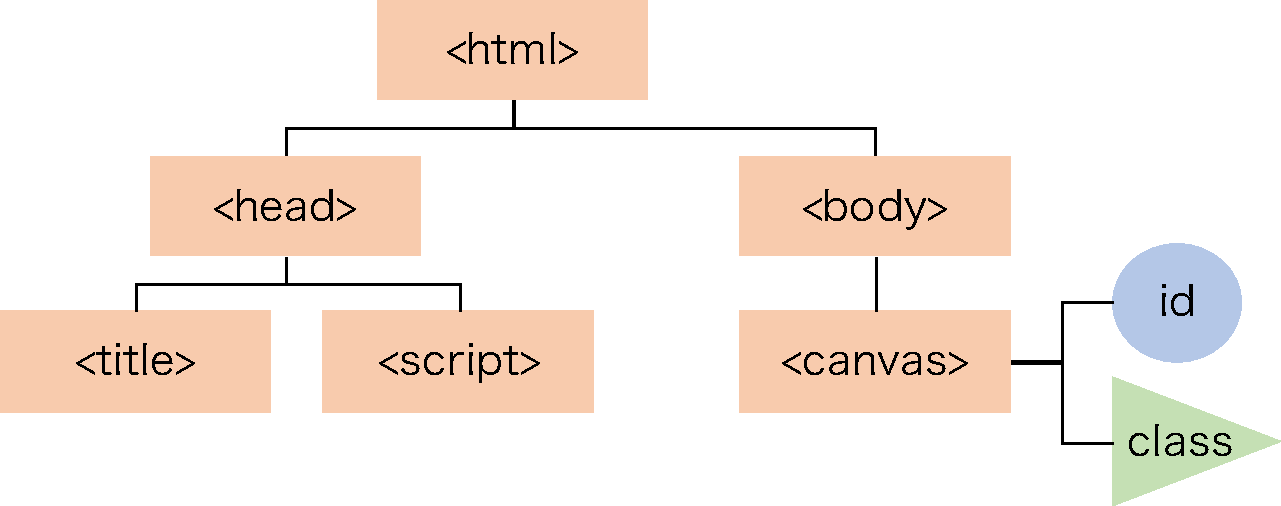
\includegraphics[width=100mm]{DOM.pdf}
 \end{center}
 \caption{DOMツリーのイメージ}
 \label{fig:DOM}
\end{figure}

\subsection{Canvas}
canvasタグとは,HTML5で新しく追加された要素の一つであり,図を描画するために策定された仕様である.従来HTML上で図を表現するには画像に置き換えるか,条件に応じて表示する図を変化させる必要があった.アニメーションを実現するにはFlash やJavaアプレットが使用されてきた.

それに対し,canvasタグはHTML5に対応するブラウザ内でプラグインを利用することなく,JavaScriptベースで図を描画することが可能である.
\newpage

%プログラミング言語
\section{プログラミング言語}
プログラミング言語とは,コンピュータのプログラムを記述する言語であり,ソフトウェアのアルゴリズムを記述するための言語である.

本章では本論文で使用したプログラミング言語について述べる.
\subsection{プログラミング言語の種類}
プログラミング言語はいくつかに分類することができる.

ソースコードを機械語へ翻訳する方法は2種類ある.1つはソースコードを実行する前に機械語へ変換を行うコンパイラ型である.特徴として始めにコンパイルを行うため,コンパイルする時間を有するが,コンパイル後は行う必要性がないことからプログラムの実行速度が速くなる.

もう1つはプログラムを1行ずつ機械語に翻訳して実行するインタプリタ型である.インタプリタ型の特徴は直ぐに実行できるため,動作を確認しながら開発を行えることである.しかし,実行する都度機械語に翻訳するためコンパイラ型と比べ処理が遅くなる.

プログラムの構築方法によって,プログラミング言語を分類することができる.手続きを順番に記述する手続き型言語,関連するデータと手続きを1つのまとまりとして捉えるオブジェクト指向言語,プログラムを関数の組み合わせで実行する関数型言語,データ間の関係や理論を記述する記述型言語に分けられる.

%JavaScript
\subsection{JavaScript}
本研究ではJavaScriptを用いた開発を行った.そこで本章ではJavaScriptの特徴と歴史について紹介する.
\subsubsection{JavaScriptの特徴}
\begin{description}
 \item[インタプリタ型]\mbox{}\\ 
JavaScriptはインタプリタ言語である.近年のWebブラウザの多くは実行時にソースのコンパイルを行うJIT(Just In Time)コンパイラを導入したことにより,実行速度を高めている.
 \item[動的なオブジェクト指向言語]\mbox{}\\
JavaScriptはプロトタイプベースのオブジェクト指向言語である.JavaScriptのオブジェクトは後からプロパティやメソッドを動的に追加,削除することができる.
 \item[動的型付けの言語]\mbox{}\\
C++やJavaは,変数の型が実行前に決まる静的型付けの言語である.一方,JavaScriptは変数に型がなく,プログラムの実行と共に変数に納めるデータの型が動的に変更する.	   
\item[関数が第一級オブジェクト]\mbox{}\\
JavaScriptの関数はオブジェクトであり,関数の引数を渡すことができる.	   
\item[関数はクロージャを定義する]\mbox{}\\
JavaScriptの関数は自分を囲むスコープにある変数を参照することができるため,隠蔽や永続化など様々な機能を実現できる.
\end{description}
\subsubsection{JavaScriptの技術的要素}
JavaScriptの中核となる技術は,ECMAScriptによって規定されている.TC-39委員会によって標準化されECMA-262という文章で公開されている.

Webブラウザで動作するJavaScriptをクライアントJavaSctiptという.ECMAScriptによって規定されたコア言語と,Webブラウザ特有のAPI(Application Program Interface)から構成されている.また,HTML5で規定されているAPIで様々なAPIを利用することができる.

Webサーバーでは,PHPやRubYなどのプログラミング言語が広く利用されているが,近年サーバーサイドJavaScriptの利用も増加してきた.サーバーサイドJavaScriptの実行環境にはNode.jsやRhinoなどがある.

\subsubsection{ECMAScript2018の新機能}
2015年に公表されたECMAScript6から毎年使用を改定することとなったため,ECMAScript2015とも呼ばれ,現在はECMAScript2018が最新である.そこで定義された新機能を表\ref{tab:EC2018}に示す.

\begin{table} [h]
\centering
\caption{ECMAS2018にて改定された主な内容}
	\begin{tabular} {| c | l |} \hline
	オブジェクトのRest/Spread プロパティ &  オブジェクト内に別のオブジェクトを展開する構文を実装\\ \hline
	Promise.prototYpe.finallY &  プロミスの成否に関わらず処理を行うメソッド\\ \hline
	テンプレートリテラルの改修 &  タグ付きのテンプレートリレラルの場合エラーが出ない\\ \hline
	正規表現 & sオプションを付けることで改行文字に対応など \\ \hline
	AsYnchronous Iterators & 非同期のイテレータやジェネレータが利用可能 \\ \hline
	\end{tabular} 
	\label{tab:EC2018}
\end{table}

\subsubsection{JavaScriptの歴史}
JavaScriptは,1995年にNetscape Communications社のBrendan Eichによって開発されNetscape Navigator 2.0にて実装された.1996年,Microsoft社のInternet EXploer 3.0に搭載され急速に普及した.

JavaScriptの黎明期には各々が独自の拡張を行ったため,ブラウザ間での互換性が低く,各ブラウザに対応したコードを書く必要があった.1997年からECMAScriptによる標準化が進められ,各ブラウザはその使用を実装したため,ブラウザ間の互換性の問題は解消している.

JavaScript本来の言語仕様を解説した本がなかったことや,当時のブラウゼ機能の処理が低いことから,プログラマが本気で取り組む言語ではないと考えられていた.しかし,AjaXという非同期通信技術を使い,デスクトップアプリケーションと遜色ないソフトウェアの登場によりその認識が薄れ,理解されるようになった.2008年からHTML 5.0の策定が始まり,JavaScriptによるWebアプリケーションを作るための様々なAPIが規定され,ブラウザの高品質化が進み,JavaScriptが普及していった.

\subsubsection{実行方法}

\begin{Large}
setInterval()
\end{Large}

setInterval()は一定時間間隔を開けてコードを繰り返し行うメソッドである.経過する時間はミリ秒[ms]で指定される.

setInterval()は前の処理が完了したか確認せずに次の処理を開始するため重たい処理を行うため予期せぬ動作をする場合がある.
\begin{lstlisting}[frame=single]
setInterval( 関数 , 遅延時間指定 [ , 引数 ] )
 \end{lstlisting}


\begin{Large}
requestAnimationframe()
\end{Large}

requestAnimationFrame()はブラウザにアニメーションを行うことを知らせ,指定した関数を呼び出してアニメーションを更新するメソッドである.

画面上でアニメーションの更新準備が整ったときに呼び出される.つまり,ブラウザの再描画が実行される前に呼び出されることを要求する.通常毎秒60回だが,W3Cの勧告に従い,ディスプレイのリフレッシュレートに従う.そのため,タブに隠れたりすると描画の回数が少なくなる.

\begin{lstlisting}[frame=single]
requestAnimationFrame( 関数 )
 \end{lstlisting}
 
%WebWorker
\subsection{WebWorker}
WebWorkerとはHTML 5.0で規定されたAPIの一つである.JavaScriptはシングルスレッドの言語のため処理が実行されているときは,他の処理は保留される.WebWorkerは特定の処理をマルチスレッドで実行するAPIである.これによって高負荷の処理によって処理が中断される問題が解消される.WebWorkerで並列に実行されるスレッドをワーカーと呼び,メインスレッドとワーカーとは異なるグローバルオブジェクトを持ち互いのグローバルオブジェクトを参照することはできない.

\subsubsection{WebWorkerの実装方法}
WebWorkerを利用するにはワーカーの定義,データの送信,ワーカーでデータを受信.ワーカーでデータを送信,ワーカーのデータを受信の5つの作業が必要となってくる.
ワーカーを定義するJavaScriptのファイルが必要となる.そこでワーカーオブジェクトを生成する.
\begin{lstlisting}[basicstyle=\ttfamily\footnotesize, frame=single]
var worker = new Worker('worker.js');
 \end{lstlisting}
ワーカーのファイルは相対URLと絶対URL両方用いることができる.絶対URLの場合は同一生成元である必要がある.


postMessageを使うことでワーカーにメッセージを送ることができる.WindowオブジェクトやDocumentオブジェクトは送信できない.
\begin{lstlisting}[basicstyle=\ttfamily\footnotesize, frame=single]
worker.postMessage("message");
 \end{lstlisting}

ワーカーでメッセージを受信するにはグローバルオブジェクトにonmessageイベントハンドラを登録しておく.送信されたデータはイベントオブジェクトのdataプロパティに格納される.
\begin{lstlisting}[basicstyle=\ttfamily\footnotesize, frame=single]
addEventListerner('message', fuction(e) { 
	var  message = e.data;
};
 \end{lstlisting}

ワーカーで処理したデータをメインスレッドに送信するには,グローバルオブジェクトのpostmessageを呼び出す.
\begin{lstlisting}[basicstyle=\ttfamily\footnotesize, frame=single]
postmessage('message');
 \end{lstlisting}

メインスレッドでメッセージを受信するには,Workerオブジェクトにmessageイベントハンドラを登録しておき,送信されたデータはdataプロパティに格納されている.
\begin{lstlisting}[basicstyle=\ttfamily\footnotesize, frame=single]
worker.onmessage = function(e) {
	var message = e.data;
};
 \end{lstlisting}

%OffscreenCanvas
\subsection{OffscreenCanvas}
OffscreenCanvasとは,従来行えなかったWebWorkerでの描画処理を可能とするAPIである.

従来はJavaScriptで動的に描画を行うかメインとなるスレッドで描画するしか方法がなかった.WebWorkerの登場により,別スレッドに計算処理を分離することで処理を高速化させていた.しかし,メインスレッドの描画速度は上がらないため,3Dなど描画対象が多くなるとイベントが大量に発生し,他の処理が中断し結果として動作が遅いということがあった.しかし,OffscreenCanvasの登場でそれらの現象の改善が期待されるようになった.また,OffscreenCanvasは処理と描画を同一のスレッドで行うことで,WebWorkerでは処理後に必要としたメインへデータの送信が要らなくなった.

Webブラウザにおいて本機能が標準で行えるようになったのは2018年9月にリリースされたChrome 69からであり,対応しているブラウザは,2019年1月の時点でChromeの他にChrome for Android,OperaとOpera for AndroidがOffscreenCanvasに対応している.また,実験的かつ,機能が限定的ではあるが,FirefoX,FirefoX for AndroidとAndroid Brower も対応している.

\subsubsection{OffscreenCanvasの実装法方}
まず,WebWorkerと同様にワーカーを定義する必要がある.
\begin{lstlisting}[basicstyle=\ttfamily\footnotesize, frame=single]
var worker = new Worker('worker.js');
 \end{lstlisting}
 
 次にCanvas要素の描画コントロールをOffscreenCanvasに移譲する.
 \begin{lstlisting}[basicstyle=\ttfamily\footnotesize, frame=single]
var offscreenCanvas = canvas.transferControlToOffscreen();
 \end{lstlisting}
 
 データをpostMessageを用いてワーカーに送る
 \begin{lstlisting}[basicstyle=\ttfamily\footnotesize, frame=single]
worker.postMessage({canvas: offscreenCanvas}, [offscreenCanvas]);
 \end{lstlisting}
 
 最後にワーカーで送信されたデータを受け取る.ワーカーと同様にdataに送信されたデータが格納されている.
  \begin{lstlisting}[basicstyle=\ttfamily\footnotesize, frame=single]
 addEventListerner('message',fuction(e) { 
  const offscreenCanvas = event.data.canvas;
}
 \end{lstlisting} 
これら一連の処理を行った後は,ワーカーであることを意識せずに,演算,描画を行う事ができるため,1つのファイルでrequestAnimationFrameやsetIntervalを用いたアニメーションを制作することが可能である.
また,HTMLのcanvas要素で使用されるメッソドを用いることは可能なため,従来のキャンバスの操作と変わらない操作性を保持している.

\newpage
%実装したシミュレータ
\section{開発したシミュレータ}
\label{sec:kaihatsu}
本章では実際に開発したシミュレータについて論じる.
\subsection{開発したシミュレータ}
本研究では昨年度本学卒業論文である「GPU利用によるシミュレータ教材の演算速度」で用いられたソースコードを拡張することで開発を行う.

\subsection{開発したシミュレータ教材}
図\ref{fig:sim}は複数の音源から発せられる音場を可視化するシミュレータ教材である.
昨年度本学の卒業研究である「GPU利用によるシミュレータ教材の演算速度」を基に開発を行った.

本研究ではWorkerなどを使用せず,素のJavaScriptで開発を行った手法を手法1とし,シェーダでGPUに移植を行った手法を手法2とする.WebWorkerを利用し開発を行った手法を処理3とする.OffscreenCanvasを利用し開発を行う手法を手法4とする.

図\ref{fig:sim}は開発を行ったシミュレータの画像である.手法3,手法4は開発したシミュレータ教材のCanvas要素を縦に2分割した.

\begin{figure}[htbp]
 \begin{minipage}{0.5\hsize}
  \begin{center}
   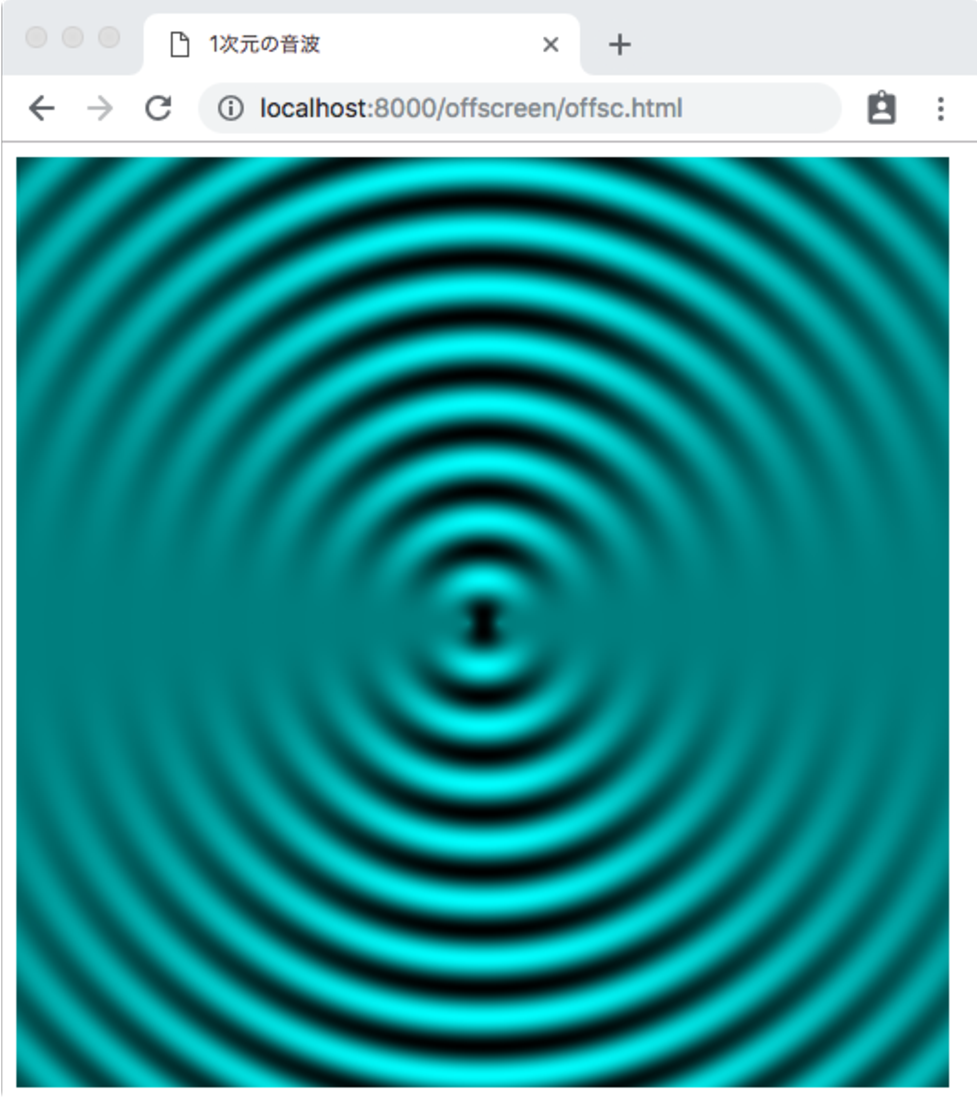
\includegraphics[width=50mm]{sim.pdf}
  \end{center}
  \caption{開発したシミュレータ}
  \label{fig:sim}
 \end{minipage}
 \begin{minipage}{0.5\hsize}
  \begin{center}
   \includegraphics[width=50mm]{kYouzai.pdf}
  \end{center}
  \caption{開発したシミュレータ教材}
  \label{fig:sim2}
 \end{minipage}
\end{figure}

図\ref{fig:sim2}は手法4をリアルタイムで数値の変更を可能としたシミュレータ教材である.

手法1ではHTMLからCanvas要素を受信し,音場の計算と描画を行った.
手法3では手法1の音場の計算をサブスレッドで行い描画をメインスレッドで行った.
手法4では手法1の音場の計算と描画をサブスレッドで行うことで,演算と描画2つの負荷を分散させた.

\subsection{計測方法}
本章では計測を実施した環境とその方法を記載する.
\subsubsection{計測環境}
本研究では以下のスペックのパソコンを用いて計測を行った.
\begin{table} [h]
\centering
\caption{計測環境}
	\begin{tabular} {| c | c |} \hline
	OS & macOS High Sierra(10.13.6) \\ \hline 
	メモリ & 32GB \\ \hline
	CPU & Intel Core i5 3.2GHz (4コア) \\ \hline
	GPU & NVIDIA GeForce GT 775M \\ \hline
	ブラウザ & Google Chrome 71.0.3578.98(64ビット) \\ \hline
	\end{tabular} 
	\label{tab:tab1}
\end{table}

\subsubsection{計測方法}
本研究ではそれぞれ1,000回計算するごとに費やした時間を計測,10,000回計算を行い,1,000ごとの時間と,10,000回計算を行うのに有した時間を測定した.

処理に費やした時間の比を式(\ref{eq:cal})に当てはめて求めた.

WebWorkerとOffscreenCanvasはキャンバスを分割し表示させているため,左右で計測時間が異なる.したがって,WebWorkerとOffscreenCanvasはより計測時間を費やしたキャンバスを参照する.
\begin{equation}
 時間比 = \frac { 各手法が10,000回演算するのに費やした時間 [s]} { 手法1が10,000回演算するのに費やした時間[s] } 
\label{eq:cal}
\end{equation}

手法3,手法4はCanvas要素を分割したため,左右の演算速度の差の計測を行う.
\newpage

%結果
\section{実験結果}
本章では\ref{sec:kaihatsu}章で示した計測方法を基に得られた結果を記す.

本章では演算時間の他に手法3,手法4のCanvasごとに生じた演算時間の差や演算回数による演算時間の変化を述べる.また,手法ごとに生じたソースコードの追加箇所についても言及する.
\subsection{演算時間}
\label{sec:sokudo}
setInterval()を用いて実行した.各手法10,000回演算実行するのに費やした時間と時間比を表\ref{tab:hi}に示す.

\begin{table}[htb]
\centering
\caption{演算時間と時間比}
\label{tab:hi}
  \begin{tabular}{| c | c | c |} \hline
    手法 & 演算時間[s] & 時間比 \\ \hline \hline
    手法1 & 206.6 & 1 \\ \hline
    手法2 & 128.7 & 0.622 \\ \hline
    手法3 & 98.1 &  0.796 \\ \hline
    手法4 & 164.4 & 0.475 \\ \hline
  \end{tabular}
\end{table}


図\ref{tab:hi}より,手法2\UTF{FF5E}4全て手法1を上回る処理速度を実現できた.ディスプレイのリフレッシュレートより高い処理速度を実現できたため,速度面において有用であると言える.

\subsection{Canvas要素の分離による左右の処理速度の差}
\label{sec:sa}
\ref{sec:sokudo}により速度面の有用性は証明できた.しかし,手法3と手法4においてはCanvas要素を2分割しているため,左右のズレが大きくてはシミュレータとしての体を成すことはできない.したがって,本章ではキャンパスを分割したことによるズレの検証を行う.
検証方法は各手法10,000回計測した際に費やした時間をそれぞれのキャンバスごとに計測し,左右のズレを検証する.

\begin{table}[htb]
\centering
\caption{手法3,手法4のCanvasごとの演算時間の差}
\label{tab:sa}
  \begin{tabular}{| c || c | c | c | c |} \hline
    手法 & 手法3(左) & 手法3(右) & 手法4 (左) & 手法4(右) \\ \hline
    演算時間[s] & 164.4 & 164.4 & 98.0 & 97.3 \\ \hline
     差[s] & \multicolumn{2}{ c|}{0} & \multicolumn{2}{c|}{0.7}  \\ \hline
  \end{tabular}
\end{table}


表\ref{tab:sa}より手法4の差は大きいと言える.本研究では生産性の検証を主としているため,手法4においては各サブスレッドごとに同期処理を行わなかったことが原因であると推測する.

したがって,描画結果をメインスレッドに送り同期処理を行うことで差を埋めることができると考える.
また,本研究ではsetIntervalを実行に用いたが,requestAnimationFrameを用いることによりCanvasごとの演算時間の差を埋めることができると考える.

\subsection{1000回ごとの演算時間}
図\ref{fig:henka}に各種法が1000回の演算に費やした時間の変化を示す.

各手法に演算回数による処理時間の変化は見られなかった.

\begin{figure}[htbp]
 \begin{center}
  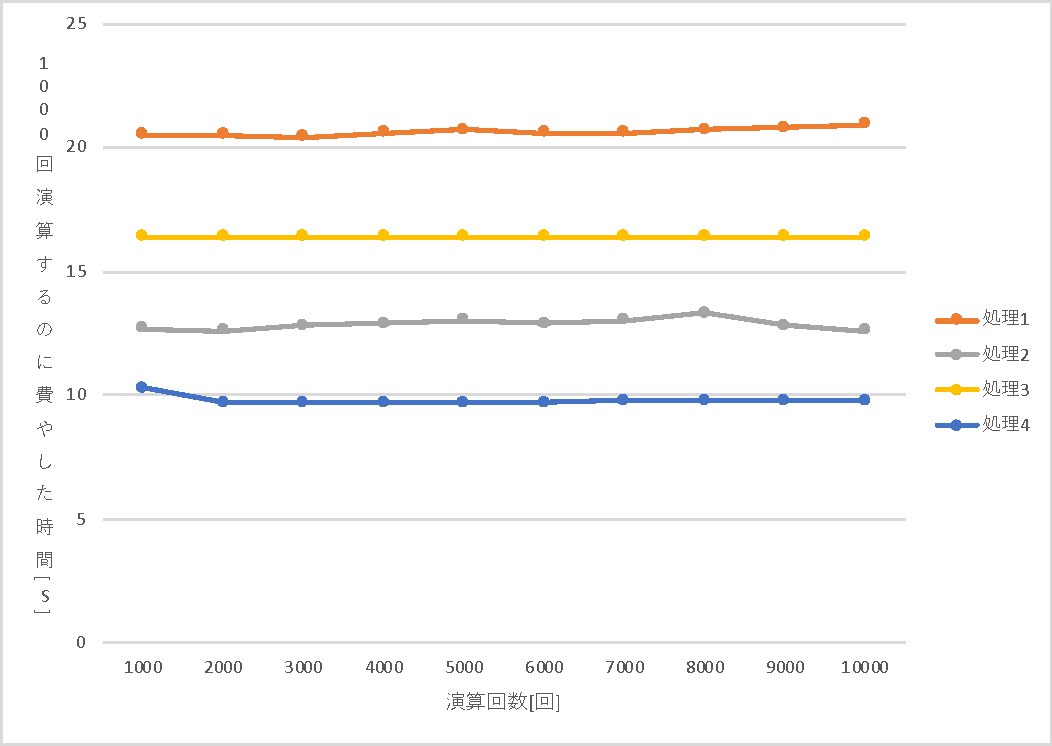
\includegraphics[width=100mm]{henka.pdf}
 \end{center}
 \caption{演算回数によるパフォーマンスの変化}
 \label{fig:henka}
\end{figure}
\newpage

\subsection{各手法による実装の違い}
本章では各手法の生産性の観点からOffscreencanvasの有用性の検証を行う.
\subsubsection{手法1}

図\ref{fig:cpu}は手法1のフローチャートである.HTMLからCanvas要素を取得した後,演算部分では,複数の音源から発せられる音の音場の計算を行う.計算は1フレーム,Canvasのサイズだけ行う.
演算で得られた情報を基に描画を行う.この手順を繰り返し行うことでアニメーションさせている.
\begin{figure}[H]
 \begin{center}
  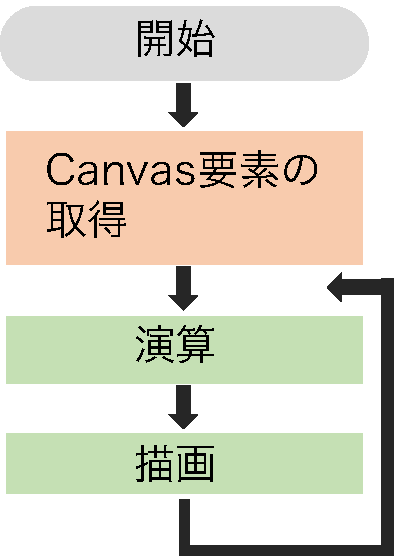
\includegraphics[width=40mm]{cpu_chart.pdf}
 \end{center}
 \caption{手法1のフローチャート}
 \label{fig:cpu}
\end{figure}

\subsubsection{手法3}
図\ref{fig:worker}は手法3のフローチャートである.WebWorkerでは描画を行うことができないため図\ref{fig:cpu}の演算と描画の処理が分断される.

したがってまず,サブスレッドへCanvas要素などのパラメータを送信を行う.その後,サブスレッドで受信したデータを基に演算を行い結果を再度メインスレッドへ送信する.最後にメインスレッドでは各サブスレッドの同期を行い,描画を実行する.この処理を繰り返し行うことで,処理を継続することが可能となった.
ソースコードは処理と描画が分断されるため,存在していたコードを分ける必要があった.

%手法3の図
\begin{figure}[H]
 \begin{center}
  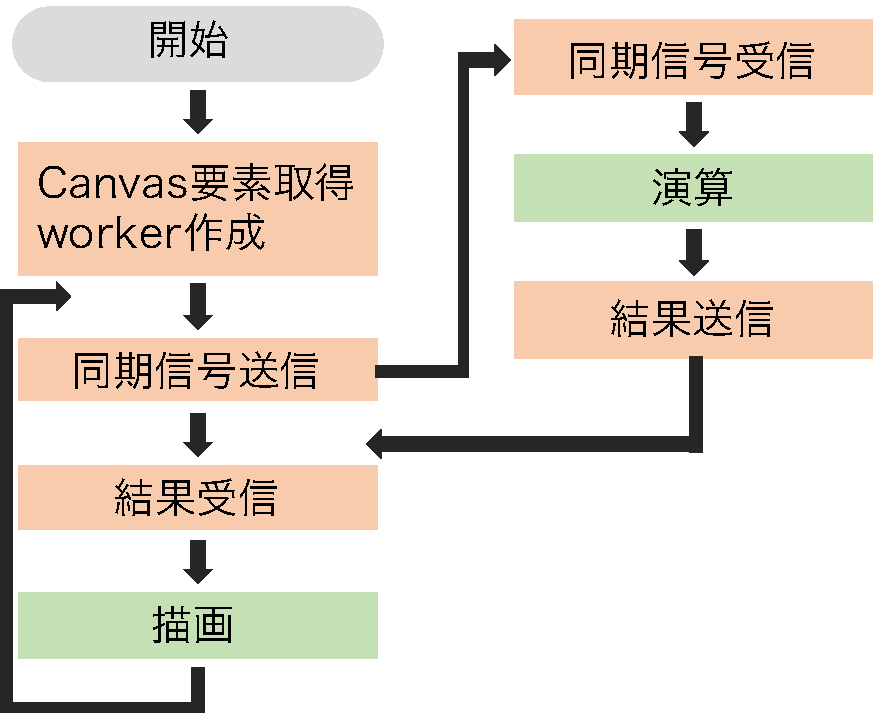
\includegraphics[width=70mm]{worker_chart2.pdf}
 \end{center}
 \caption{手法3のフローチャート}
 \label{fig:worker}
\end{figure}

\subsubsection{手法4}
図\ref{fig:offsc}は手法4のフローチャートである.OffscreenCanvasはWebWorkerを利用し,従来サブワーカーでは行えなかった描画を可能とするAPIである.

したがって,手法3と同様にサブスレッドへCanvas要素などのパラメータの送信を行う.サブスレッド内で描画まで行えるため手法1の演算の結果をメインスレッドへ送る必要がなかった.サブワーカー内で演算と描画が行えるため,処理1を大きく変更することなく移植を可能とした.
%手法4の図
\begin{figure}[H]
 \begin{center}
  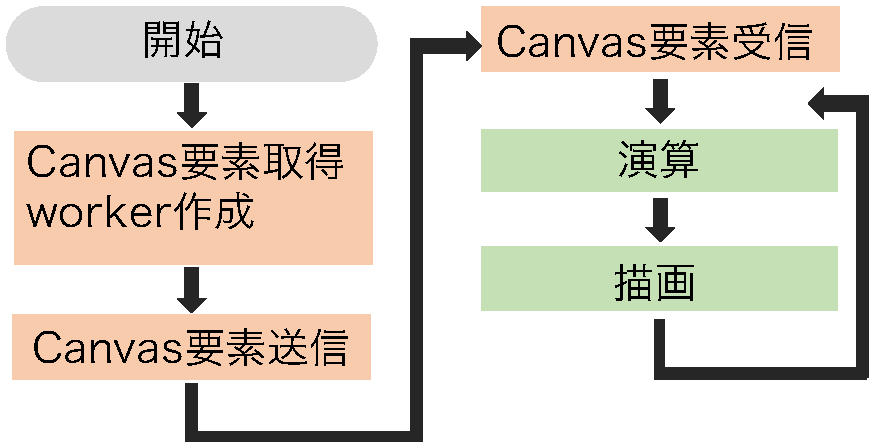
\includegraphics[width=80mm]{offsc_chart2.pdf}
 \end{center}
 \caption{手法4のフローチャート}
 \label{fig:offsc}
\end{figure}

\newpage


\section{結言}
近年のe-Learningの普及により高い処理速度と高い生産性を両立させた開発手法が求められている.

本研究室ではシミュレータ教材を対象とした高速化手法の提案を行っている.それらの研究では処理速度の向上は得られたが,設計やデバックなど実装が容易でなかった.

そこでWebWorkerを利用しながら描画もサブスレッドで完結されることのできるOffscreenCanvasを用いた開発を行い処理速度と生産性の観点から検証を行った.

OffscreenCanvasを利用することで高い処理速度が得られる一方で,新たに書き足す必要性があることがわかった.

既存のシミュレータ教材へOffscreenCanvasを適用する場合は一連の処理をサブスレッドに移植するだけで実装が可能なため,ソースコードを大きく変更する必要がなく,実装が容易であると結論づける.

欠点として対応しているブラウザの

今後はOffscreenCanvasに対応したブラウザが増加するにあたり,OffscreenCanvasを利用したシミュレータ教材が増加していくことが考えられる.
\newpage

\section{謝辞}
本研究の遂行及び本論文の制作に当たり,助言をくださった須田研究室の仲間に深く感謝の意を表します.そして,本論文の制作に当たり多大なるご指導及びご助言をいただきました須田宇宙准教授に深く感謝いたします.
\newpage

\section{参考文献}
\begin{thebibliography}{99}
\bibitem{book} ecma INTERNATIONAL:"EECMAScript\UTF{00AE}2018 Language Specification\" , url{https://www.ecma-international.org/ecma-262/9.0/indeX.html}(参照:2019年1月15日)
\bibitem{book}磯 博:"プログラミングの教養から言語仕様,開発技法までが正しく身につく徹底マスターJavaScriptの教科書",SB Creative,2017年3月25日
\bibitem{book}大島 篤:"見てわかるパソコン解体新書",SB Creative,2001年4月30日
\bibitem{book}大島 篤:"見てわかるパソコン解体新書 vol3",SB Creative,2001年4月30日
\bibitem{book}豊田 政弘 :"音響サイエンスシリーズ14 FTDT法で見る音の世界",コロナ社,2015年12月16日
\bibitem{book}Hisa Ando:"GPUを支える技術 超並列ハードウェアの快進撃[技術基礎]",技術評論社,2017年7月13日
\bibitem{book}小山田 耕二,岡田 賢治:"CUDA高速GPUプログラミング入門",秀和システム,2010年3月25日
\bibitem{book}菅原 愛子:"Web Workerを利用したシミュレータ教材の開発",平成25年度卒業論文,2014年1月30日
\bibitem{book}中嶋 大貴:"GPU利用によるシミュレータ教材の演算速度",平成29年度卒業論文,2018年1月29日
\end{thebibliography}
\newpage

%プログラム
\section{付録 制作したプログラム}
\subsection{手法1}
\lstinputlisting[caption=CPU.html] {01-program/01/CPU.html}
\newpage
\lstinputlisting[caption=manY-source.js] {01-program/01/manY-source.js}
\newpage

\subsection{手法2}
\lstinputlisting[caption=GPU.html] {01-program/02/GPU.html}
\newpage
\lstinputlisting[caption=manY-source-gpu.js] {01-program/02/manY-source-gpu.js}
\newpage

\subsection{手法3}
\lstinputlisting[caption=Worker.html] {01-program/03/Worker.html}
\newpage
\lstinputlisting[caption=main.js] {01-program/03/main.js}
\newpage
\lstinputlisting[caption=worker.js] {01-program/03/worker.js}
\newpage

\subsection{手法4}
\lstinputlisting[caption=offsc.html] {01-program/04/offsc.html}
\newpage
\lstinputlisting[caption=main.js] {01-program/04/main.js}
\newpage
\lstinputlisting[caption=manY-source.js] {01-program/04/manY-source.js}
\newpage
\lstinputlisting[caption=manY-source.js] {01-program/04/manY-source1.js}
\newpage

\subsection{手法4の数値変更}
\lstinputlisting[caption=offsc.html] {01-program/04/offsc.html}
\newpage
\lstinputlisting[caption=main.js] {01-program/04-2/main.js}
\newpage
\lstinputlisting[caption=manY-source.js] {01-program/04-2/manY-source.js}
\newpage
\lstinputlisting[caption=manY-source.js] {01-program/04-2/manY-source1.js}
\newpage
\lstinputlisting[caption=nYlon.js] {01-program/04-2/nYlon.js}
\newpage
\end{document}
